\chapter{Objetivos y metodología}\label{cap.objetivos}
En este capítulo se expondrá de manera detallada el objetivo principal de este proyecto así como la metodología utilizada para su desarrollo. También se incluirá un plan de trabajo donde se explican las diferentes etapas seguidas para la realización del proyecto.

\section{Objetivos}

El objetivo principal de este trabajo es llevar a cabo dos nuevas prácticas para la plataforma JdeRobot-Academy de manera que se consiga que los alumnos que las realicen solo tengan que concentrarse en la parte de programación de robots. Además, gracias a la realización de estas prácticas el alumno adquirirá tanto conocimientos sobre programación de Python en robótica como conocimientos relacionados con el tratamiento digital de la imagen y la toma de decisiones. \\

El objetivo de la práctica ``Reconocimiento de la señal stop'' es conseguir que un coche autónomo sea capaz de reconocer una señal de stop situada a lo largo de una carretera, gracias a la cámara que lleva situada en el capó, y después, frene. Además, tiene que ser capaz de reconocer si se acercan otros coches y en caso negativo volver a arrancar. Y por último, tiene que hacer un giro a la izquierda o a la derecha de manera aleatoria. \\

En la práctica ``Aspiradora autónoma con autolocalización'', el objetivo es lograr que un robot aspirador sea capaz de barrer la mayor superficie posible de un apartamento en un tiempo limitado. Para ello, el alumno tiene que hacer uso de la capacidad de autolocalización de la aspiradora y del mapa de la casa.

\section{Metodología}
Como parte principal de la metodología se han ido acordando reuniones semanales con el tutor y los miembros del grupo de trabajo. En estas reuniones, el tutor iba revisando el trabajo realizado y marcando nuevos objetivos para la semana siguiente. Además, servían para corregir fallos y comentar las dudas que iban surgiendo a lo largo de los meses de trabajo. Gracias a esto, se podía avanzar de manera más fluida en la realización del proyecto. \\

También se ha desarrollado una bitácora en la Wiki de JdeRobot donde cada semana se redactaban los avances realizados y se añadían vídeos para mostrar los resultados obtenidos. \\

Conjuntamente a estas herramientas se ha utilizado un repositorio de Git Hub. En este repositorio se encuentra el código empleado en las prácticas, tanto el código de la infraestructura como el de las soluciones.
El desarrollo de trabajo que se ha seguido es el modelo de desarrollo en espiral. Este modelo consiste en una serie de ciclos o iteraciones que se repiten en forma de espiral como se muestra en la Figura~\ref{fig.espiral}.

\begin{figure}[H]
  \begin{center}
    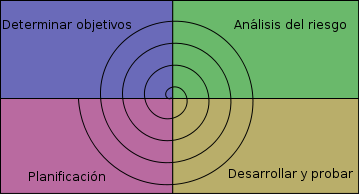
\includegraphics[width=0.6\textwidth]{figures/Objetivos/espiral.png}
		\caption{Metodología en espiral}
		\label{fig.espiral}
		\end{center}
\end{figure}

Cada ciclo consta de cuatro fases que son las siguientes:
\begin{itemize}
	\item Determinar objetivos: en esta fase se definen los objetivos que se deben de llevar a cabo para que una vez completados se pueda dar por finalizado el ciclo.

	\item Análisis del riesgo: en la segunda fase se evalúa que problemas es posible encontrarse al empezar el desarrollo.

	\item Desarrollar y probar: en la tercera fase, una vez evaluados los riesgos se procede al propio desarrollo del trabajo realizando distintas pruebas para conseguir el mejor resultado.

	\item Planificación: en esta última fase se valoran los resultados obtenidos y se planifican los siguientes etapas del proyecto.
\end{itemize}

No existe un número fijo de iteraciones, deben de llevarse a cabo tantas como sean necesarias hasta completar el trabajo. \\

La adaptabilidad en el diseño del modelo de espiral en la ingeniería de software se adapta a cualquier número de cambios, que pueden ocurrir durante cualquier fase del proyecto, permitiendo minimizar los riesgos y realizar un buen desarrollo del trabajo.

\section{Plan de trabajo}

Para lograr los objetivos ya descritos, se han seguido las siguientes etapas:
\begin{itemize}
	\item Familiarización del entorno JdeRobot, mediante la descarga e instalación del software de JdeRobot además de las distintas dependencias necesarias para el correcto uso de JdeRobot. En esta etapa también se llevó a cabo la resolución de algunas prácticas anteriores de JdeRobot-Academy relacionadas con las prácticas a desarrollar.

	\item Familiarización del simulador Gazebo. En esta etapa se han estudiado distintos ejemplos disponibles en la web de Gazebo y de JdeRobot. Además, se han comprendido los distintos plugins necesarios para el desarrollo del trabajo lo que implicó un aprendizaje básico del lenguaje de programación C++.

	\item Crear los mundos y plugins necesarios de Gazebo.  Se modificaron distintos plugins ya creados para adaptarlos a las prácticas que se iban a desarrollar. También se diseñaron los mundos que se han utilizado en cada ejercicio incluyendo en dichos mundos tanto los modelos de objetos y obstáculos como los de los robots y coches.

	\item Desarrollar la infraestructura, que consistirá principalmente en crear la interfaz gráfica, utilizando la herramienta PyQt5, para que el alumno pueda resolver las prácticas de manera más sencilla e intuitiva.

	\item Desarrollar un evaluador automático, para que el alumno sepa de manera automática que nota ha obtenido con el código que programe. Este evaluador medirá distintos parámetros y calculará una nota final. También ha sido necesario el uso de la herramienta PyQt5.

	\item Realizar las soluciones. En esta etapa se ha realizado un algoritmo por cada práctica.

	\item Redactar los enunciados, donde se explica el contenido de cada práctica.
\end{itemize}

